\section{Grundlagen}
In diesem Kapitel werden die wichtigsten Grundlagen erklärt, welche nötig sind um den Bericht zu verstehen.
\subsection{Grundlagen zur Energieübertragung}
In diesem Unterkapitel werden die Grundlagen zur Energieübertragung erläutert. Im wesentlichen beinhaltet dies folgende Themen:
\paragraph{Flyback}
\paragraph{Kopplungsfaktor}
\paragraph{Transformator Ersatzschaltbild}

\subsection{Grundlagen zur Datenübertragung}
In diesem Unterkapitel werden die Grundlagen zur Datenübertragung erläutert. Im wesentlichen beinhaltet dies folgende Themen:
\paragraph{VARAN-Bus}

Der VARAN-Bus ist ein Echtzeit-Bussystem für die industrielle Automatisierung. Der Bus ist ein offener, herstellerunabhängiger Standard. Er verbindet Anlagen, Maschinen und Komponenten in der modernen Industrie. Das Bussystem arbeitet nach dem Manager-/Client-Prinzip. Weil der Manager die Kommunikation initialisiert, sind Paketkollisionen ausgeschlossen. Die Übertragungsschicht basiert auf dem Ethernet-Standard nach IEEE 802.3. Die verwendete 100TX Standard Ethernet Technologie erlaubt eine maximale Übertragungsgeschwindigkeit von 100MBit pro Sekunde.

\paragraph{Ethernet}

Ethernet ermöglicht den kabelgebundenen Datenaustausch in Form von Datenframes zwischen Geräten in einem lokalen Netz. Dabei gibt es verschiedene Standards für unterschiedliche Übertragungsraten. Der 100Base-TX Standard (Fast Ethernet) des VARAN-Bus erlaubt eine maximale Datenrate von 100MBit/s. Statt der Manchesterkodierung wie beim 10MBit/s-Ethernet, wird der effizientere 4B5B-Code eingesetzt. Dadurch wird eine Taktrückgewinnung aus dem Signal möglich. Durch eine zusätzliche MLT-3 Kodierung wird der Gleichspannungsanteil entfernt.

\paragraph{4B5B-Code:}
Der Leitungscode 4B5B bildet vier Nutzdatenbits auf fünf Codebits ab. Dadurch erhöht sich die codierte Bitrate um 25\%. Beim verwendeten Ethernet-Standard beträgt die codierte Symbolrate somit 125MBit/s. Bei der Abbildung auf fünf Codebits werden lange '0' oder '1'-Folgen vermieden. Dadurch wird die Taktrückgewinnung aus dem Signal verbessert. 

\paragraph{MLT-3-Code:}
Multilevel Transmission Encoding (MLT-3) ist ein Leitungscode mit drei Spannungspegeln. Diese werden mit den Symbolen (+,0,-) bezeichnet. Bei einer logischen '1' ändert sich der Spannungspegel nach der fixen Folge [0,+,0,-]. Wird eine logische '0' übertragen, ändert sich der Zustand der Leitung nicht.
\begin{figure}[h]
\centering
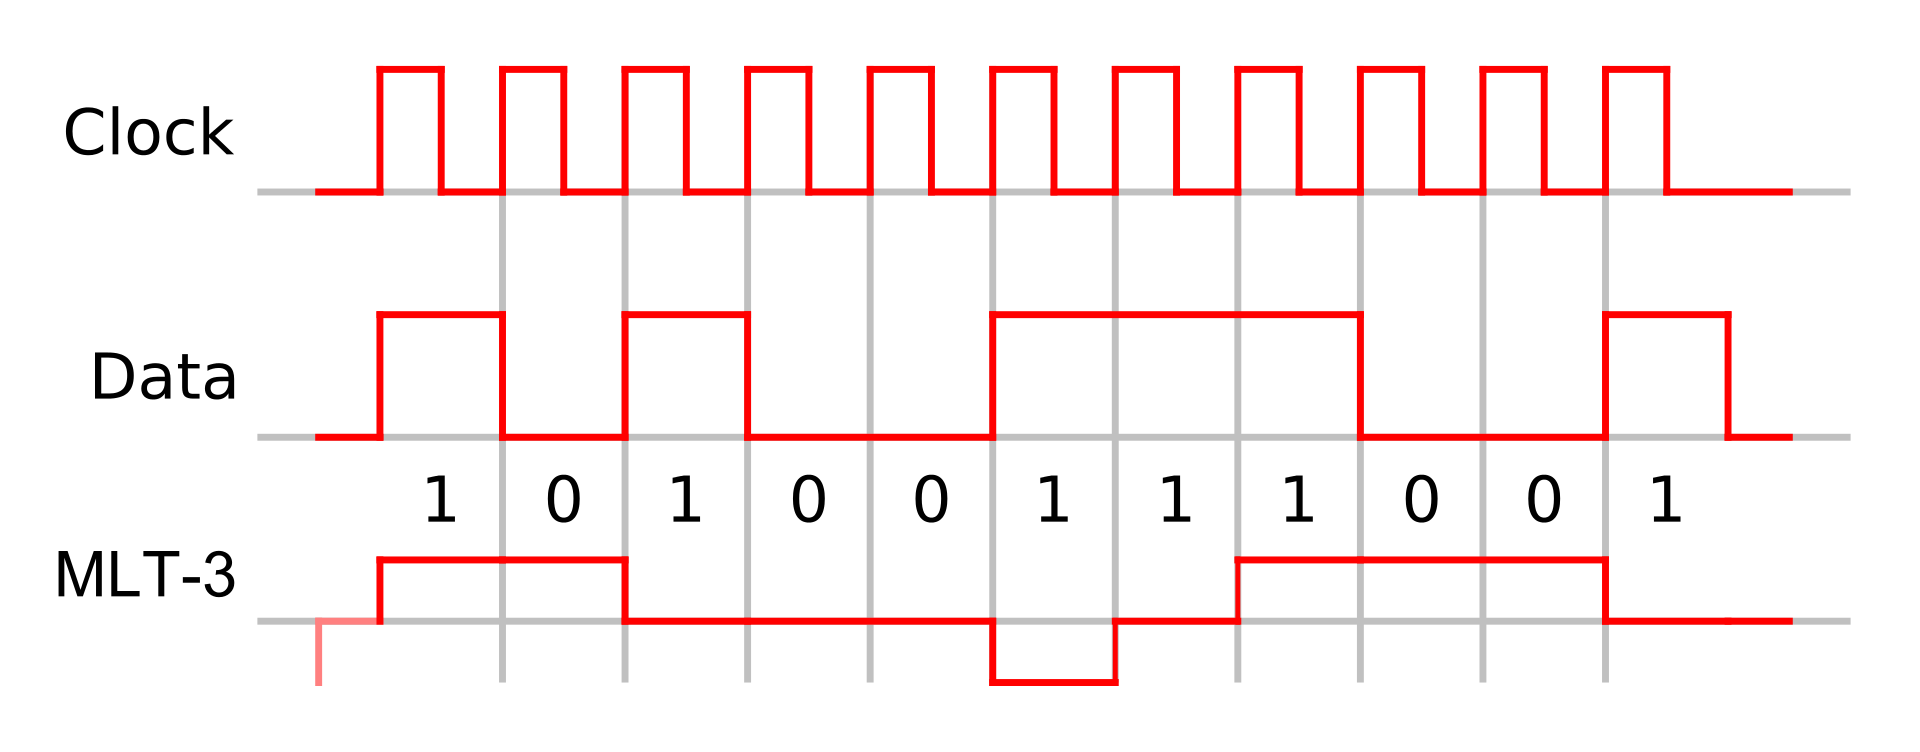
\includegraphics[width=0.8\linewidth]{MLT3encoding.png}
\caption{MLT-3 codierte Datenfolge}\label{fig:MLT3code}
\end{figure}

In einer Übertragungsschwingung werden 4 Bit übertragen. Damit reduziert sich die eigentliche Übertragungsfrequenz auf einen Viertel der Symbolrate. Die maximale Übertragungsfrequenz auf der Leitung beträgt demnach: 
\begin{equation}\label{MLT3}
f_{max}=\frac{Symbolrate}{4 Bit}=\frac{125Mbit/s}{4 Bit}=31.25 MHz
\end{equation}

\paragraph{Photodioden-Verstärker}
Photodioden sind Halbleiter-Dioden, die auftreffende Photonen in einen elektrischen Strom umwandeln. Folgende Abbildung zeigt die typische U-I-Kennlinie einer Photodiode.
\begin{figure}[h]
	\centering
	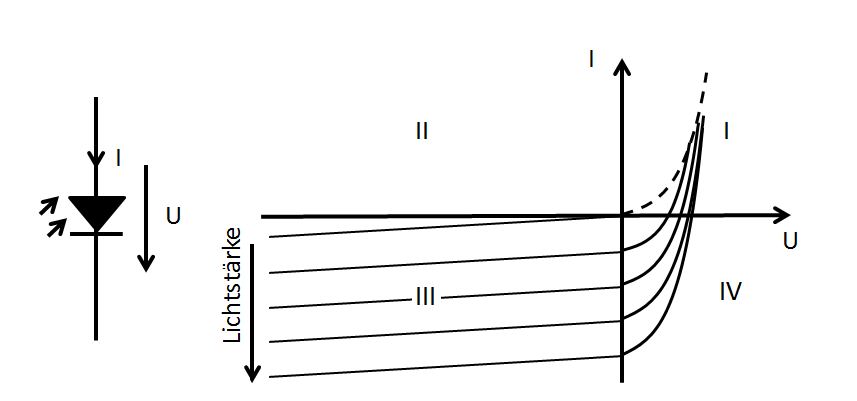
\includegraphics[width=0.8\linewidth]{Kennlinie_Photodiode.png}
	\caption{typische Kennlinie einer Photodiode}\label{fig:Kenn_Photodiode}
\end{figure}
Da im dritten Quadranten ein linearer Zusammenhang zwischen Lichtstärke und Photostrom erkennbar ist, eignet sich dieser Bereich für Sensoranwendungen und in unserem Fall auch Signalübertragungen.
Eine reale Photodiode besteht aus einer idealen Diode und einer parallel geschalteten Stromquelle. Der Strom ist abhängig von der Lichtstärke. Ein hochohmiger Widerstand stellt den Dunkelstrom der Photodiode dar. Die parasitäre Kapazität hängt primär von der Geometrie der Diode ab.
 \begin{figure}[H]
 	\centering
 	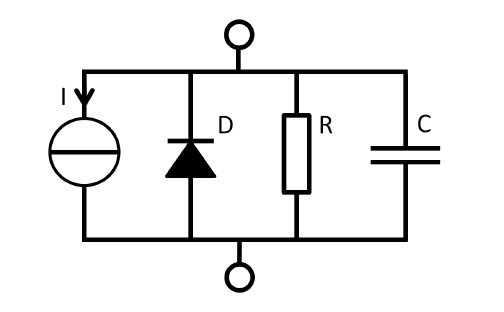
\includegraphics[width=0.8\linewidth]{Ersatzschaltbild_Photodiode.png}
 	\caption{Ersatzschaltbild einer Photodiode}\label{fig:Ersatz_Photodiode}
 \end{figure}
Für eine erfolgreiche Dimensionierung einer Schaltung, sind diese Parameter des Ersatzschaltbildes unbedingt zu beachten.\newline

Der Photostrom liegt meist im Nanoampere-Bereich und muss entsprechend verstärkt werden. Mit Hilfe eines Photodioden-Verstärkers wird der Photostrom in eine proportionale Spannung gewandelt. Meist werden dafür Transimpedanzverstärkerschaltungen eingesetzt.
\begin{figure}[h]
	\centering
	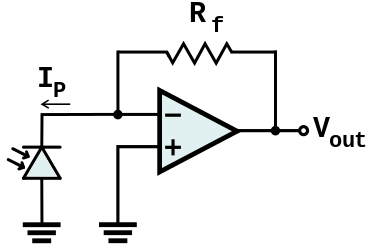
\includegraphics[width=0.5\linewidth]{Photo_Amp.png}
	\caption{Transimpedanzverstärker}\label{fig:Photo_Amp}
\end{figure}

Da die Eingänge des Verstärkers hochimpedant sind, fliesst der Photostrom $ I_{p} $ nur durch den Rückkopplungswiderstand $ R_{f} $. Am Ausgang des Verstärkers stellt sich eine positive Spannung proportional zum Strom $ I_{p} $ ein. Die Ausgangsspannung beträgt:
\begin{equation}\label{Vout_Photo}
V_{out}=R_{f} \cdot I_{p}
\end{equation}

Aus der Formel \ref{Vout_Photo} ist leicht ersichtlich, dass $ R_{f} $ dem Verstärkungsfaktor der Transimpedanzverstärkerschaltung entspricht.

